\subsection{Frontend: Benutzerschnittstelle}
Das in React geschriebene Frontend (siehe Abbildung \ref{fig:webseite}) besteht aus einer Hauptkomponente, welche aus mehreren Kindkomponenten besteht (siehe Abbildung \ref{fig:frontend}).

\textbf{Header:} Der \textit{Header} bietet die Möglichkeit, die Seite neu zu laden, Informationen über die Website zu erhalten, den Lizenztext einzusehen, den Darkmode zu aktivieren und in den Developermodus zu wechseln. Im Developermodus stehen dem Benutzer nach einer Autorisierung weitere Funktionalitäten zur Verfügung.

\textbf{Upload:} Der Uploadbereich ermöglicht es dem Benutzer ein Bild hochzuladen oder ein vorgegebenes Beispielbild auszuwählen.

\textbf{ImageView:} Die \textit{ImageView} zeigt das hochgeladene bzw. ausgewählte Bild an.

\textbf{ImageDetails:} Bei den \textit{ImageDetails} werden die zum angezeigten Bild zugehörigen Informationenen in Form eines Historgrammes angezeigt.

\textbf{Pipeline:} Bei der Komponente \textit{Pipeline} wird die aktuelle Verarbeitungskette angezeigt. Diese besteht initial nur aus dem hochgeladenen bzw. ausgewählten Bild und durch das hinzufügen weitere Bearbeitungsschritte mittels Drag and Drop erweitert werden. Ein Bearbeitungsschritt wird dabei von der Komponente \textit{PipelineStep} repräsentiert. Dieser bietet die Möglichkeit dessen Informationen anzuzeigen, die Parameter zu konfigurieren und nach erfolgreichen Durchlauf das zugehörige Zwischenergebnis anzuzeigen.

\textbf{AvailablePipelineSteps:} Bei dieser Komponente werden dem Anwender alle verfügbaren Bearbeitungsschritte angezeigt. Diese können mit der implementierten \textit{SearchBar} gefiltert werden. Ein verfügbarer Schritt, welcher mit der Komponente \textit{AvailableStep} repräsentiert wird, kann per Drag and Drop zu der Komponente \textit{Pipeline} gezogen werden. Dadurch wird die Verarbeitungskette um den ausgewählten Verarbeitungsschritt erweitert.

\textbf{StartPipeline:} Diese Komponente bietet dem Anwender die Möglichkeit, das hochgeladene bzw. ausgewählte Bild mit der erstellten Verarbeitungskette zu bearbeiten. Dabei werden alle Informationen mittels dem \textit{Controller} ans Backend weitergeleitet.

\begin{figure*}[ht]
    \centering
    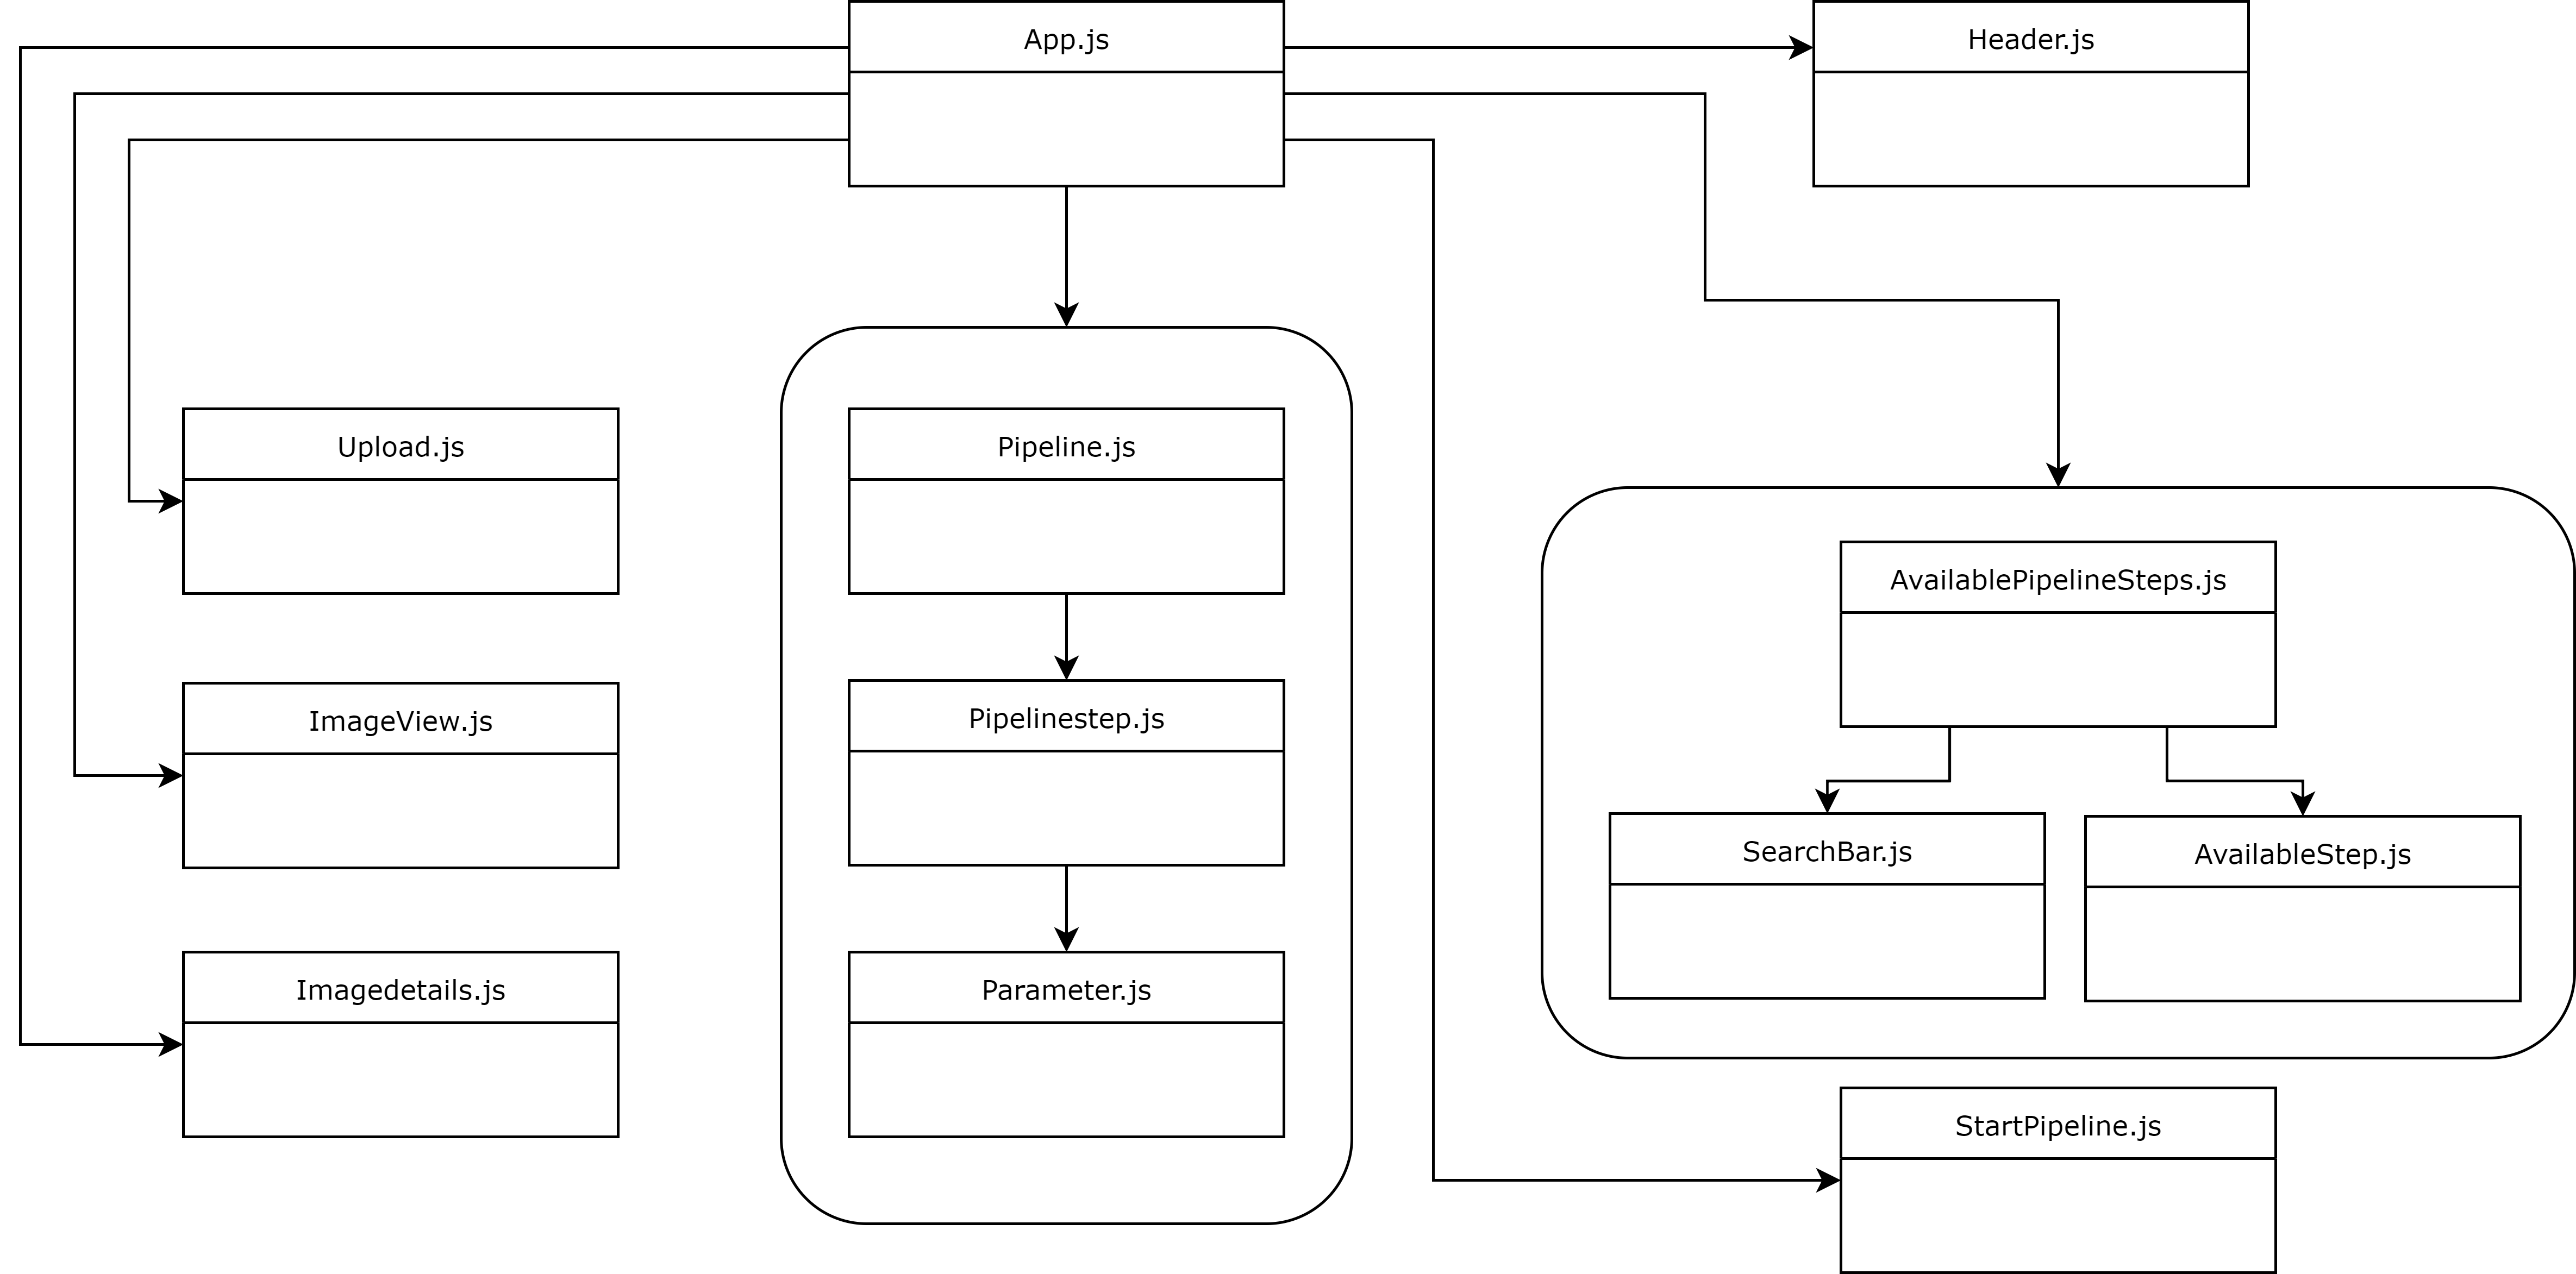
\includegraphics[width=\textwidth]{Bilder/FrontendBDCC.drawio.png}
    \caption{Übersicht der Komponenten im Frontend}
    \label{fig:frontend}
\end{figure*}